\documentclass[12pt,a4paper]{report}
\usepackage{cclicenses}
\usepackage{graphicx}
\title{Ceph Training Materials}
\author{Victor Denisov}
\date{\today}
\begin{document}
   \maketitle
\begin{abstract}
This work, ``Ceph Training Materials'', is derivative of ``Ceph Documentation'' http://docs.ceph.com/docs/master/ by Victor Denisov, used under \bysa. ``Ceph Documentation'' is licensed under \bysa by Inktank.
\end{abstract}

% Makes emph bold by default.
\makeatletter
\DeclareRobustCommand{\em}{%
  \@nomath\em \if b\expandafter\@car\f@series\@nil
  \normalfont \else \bfseries \fi}
\makeatother

\chapter{Ceph Architecture}
Ceph uniquely delivers object, block, and file storage in one unified system.
A Ceph Node leverages commodity hardware and intelligent daemons, and a Ceph
Storage Cluster accommodates large numbers of nodes, which communicate with
each other to replicate and redistribute data dynamically. All the components
of ceph storage cluster are presented on figure \ref{fig:ceph_architecture}

\begin{figure}[h]
	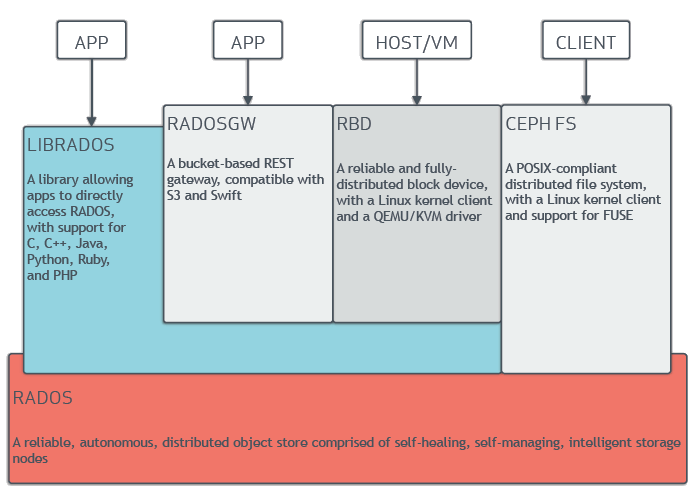
\includegraphics[scale=0.5]{stack.png}
	\caption{Ceph Architecture}
	\label{fig:ceph_architecture}
\end{figure}

\section{The Ceph Storage Cluster}


Erasure Coding

An erasure coded pool stores each object as K+M chunks. It is divided into K data chunks and M coding chunks. The pool is configured to have a size of K+M so that each chunk is stored in an OSD in the acting set. The rank of the chunk is stored as an attribute of the object.

For instance an erasure coded pool is created to use five OSDs (K+M = 5) and sustain the loss of two of them (M = 2).
Reading and Writing Encoded Chunks

When the object NYAN containing ABCDEFGHI is written to the pool, the erasure encoding function splits the content into three data chunks simply by dividing the content in three: the first contains ABC, the second DEF and the last GHI. The content will be padded if the content length is not a multiple of K. The function also creates two coding chunks: the fourth with YXY and the fifth with GQC. Each chunk is stored in an OSD in the acting set. The chunks are stored in objects that have the same name (NYAN) but reside on different OSDs. The order in which the chunks were created must be preserved and is stored as an attribute of the object (shard_t), in addition to its name. Chunk 1 contains ABC and is stored on OSD5 while chunk 4 contains YXY and is stored on OSD3.

When the object NYAN is read from the erasure coded pool, the decoding function reads three chunks: chunk 1 containing ABC, chunk 3 containing GHI and chunk 4 containing YXY. Then, it rebuilds the original content of the object ABCDEFGHI. The decoding function is informed that the chunks 2 and 5 are missing (they are called ‘erasures’). The chunk 5 could not be read because the OSD4 is out. The decoding function can be called as soon as three chunks are read: OSD2 was the slowest and its chunk was not taken into account.

Interrupted Full Writes

In an erasure coded pool, the primary OSD in the up set receives all write operations. It is responsible for encoding the payload into K+M chunks and sends them to the other OSDs. It is also responsible for maintaining an authoritative version of the placement group logs.

In the following diagram, an erasure coded placement group has been created with K = 2 + M = 1 and is supported by three OSDs, two for K and one for M. The acting set of the placement group is made of OSD 1, OSD 2 and OSD 3. An object has been encoded and stored in the OSDs : the chunk D1v1 (i.e. Data chunk number 1, version 1) is on OSD 1, D2v1 on OSD 2 and C1v1 (i.e. Coding chunk number 1, version 1) on OSD 3. The placement group logs on each OSD are identical (i.e. 1,1 for epoch 1, version 1).

OSD 1 is the primary and receives a WRITE FULL from a client, which means the payload is to replace the object entirely instead of overwriting a portion of it. Version 2 (v2) of the object is created to override version 1 (v1). OSD 1 encodes the payload into three chunks: D1v2 (i.e. Data chunk number 1 version 2) will be on OSD 1, D2v2 on OSD 2 and C1v2 (i.e. Coding chunk number 1 version 2) on OSD 3. Each chunk is sent to the target OSD, including the primary OSD which is responsible for storing chunks in addition to handling write operations and maintaining an authoritative version of the placement group logs. When an OSD receives the message instructing it to write the chunk, it also creates a new entry in the placement group logs to reflect the change. For instance, as soon as OSD 3 stores C1v2, it adds the entry 1,2 ( i.e. epoch 1, version 2 ) to its logs. Because the OSDs work asynchronously, some chunks may still be in flight ( such as D2v2 ) while others are acknowledged and on disk ( such as C1v1 and D1v1).

If all goes well, the chunks are acknowledged on each OSD in the acting set and the logs’ last_complete pointer can move from 1,1 to 1,2.

Finally, the files used to store the chunks of the previous version of the object can be removed: D1v1 on OSD 1, D2v1 on OSD 2 and C1v1 on OSD 3.

But accidents happen. If OSD 1 goes down while D2v2 is still in flight, the object’s version 2 is partially written: OSD 3 has one chunk but that is not enough to recover. It lost two chunks: D1v2 and D2v2 and the erasure coding parameters K = 2, M = 1 require that at least two chunks are available to rebuild the third. OSD 4 becomes the new primary and finds that the last_complete log entry (i.e., all objects before this entry were known to be available on all OSDs in the previous acting set ) is 1,1 and that will be the head of the new authoritative log.

The log entry 1,2 found on OSD 3 is divergent from the new authoritative log provided by OSD 4: it is discarded and the file containing the C1v2 chunk is removed. The D1v1 chunk is rebuilt with the decode function of the erasure coding library during scrubbing and stored on the new primary OSD 4.

See Erasure Code Notes for additional details.
Cache Tiering

A cache tier provides Ceph Clients with better I/O performance for a subset of the data stored in a backing storage tier. Cache tiering involves creating a pool of relatively fast/expensive storage devices (e.g., solid state drives) configured to act as a cache tier, and a backing pool of either erasure-coded or relatively slower/cheaper devices configured to act as an economical storage tier. The Ceph objecter handles where to place the objects and the tiering agent determines when to flush objects from the cache to the backing storage tier. So the cache tier and the backing storage tier are completely transparent to Ceph clients.

See Cache Tiering for additional details.
Extending Ceph

You can extend Ceph by creating shared object classes called ‘Ceph Classes’. Ceph loads .so classes stored in the osd class dir directory dynamically (i.e., $libdir/rados-classes by default). When you implement a class, you can create new object methods that have the ability to call the native methods in the Ceph Object Store, or other class methods you incorporate via libraries or create yourself.

On writes, Ceph Classes can call native or class methods, perform any series of operations on the inbound data and generate a resulting write transaction that Ceph will apply atomically.

On reads, Ceph Classes can call native or class methods, perform any series of operations on the outbound data and return the data to the client.

Ceph Class Example

A Ceph class for a content management system that presents pictures of a particular size and aspect ratio could take an inbound bitmap image, crop it to a particular aspect ratio, resize it and embed an invisible copyright or watermark to help protect the intellectual property; then, save the resulting bitmap image to the object store.

See src/objclass/objclass.h, src/fooclass.cc and src/barclass for exemplary implementations.
Summary

Ceph Storage Clusters are dynamic–like a living organism. Whereas, many storage appliances do not fully utilize the CPU and RAM of a typical commodity server, Ceph does. From heartbeats, to peering, to rebalancing the cluster or recovering from faults, Ceph offloads work from clients (and from a centralized gateway which doesn’t exist in the Ceph architecture) and uses the computing power of the OSDs to perform the work. When referring to Hardware Recommendations and the Network Config Reference, be cognizant of the foregoing concepts to understand how Ceph utilizes computing resources.


\end{document}
